\chapter{Conclusion and Future Work}
\label{chapter5}
The pipeline of this network starts from Geometric Alignment. Finger print images are not properly aligned, it depends on the how the person has placed his/her finger on the sensor, also there are various transformations which gets introduced into them which needs to be taken care before feeding those images to our main network. It can be done manually or a network \cite{Rocco2017ConvolutionalNN} can be added at the starting of our main network that aligns the images, also transforms them if required and then those images are passed to the network. Since our images are properly aligned there is still a chance that our network will not learned features of different subjects. To handle such situations hard mining is used to train our network, in which some similar as well as some most similar samples are used to train our network. Also at the end a proper indexing algorithm is required which can allow us to easily search for our target images in an efficient manner.


\begin{figure}[htbp]
\centering
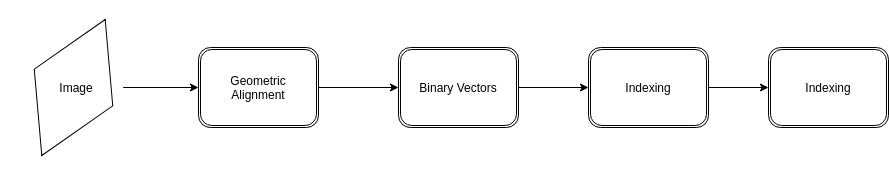
\includegraphics[scale=0.5]{./Chapter5/Figures/pipeline}
\caption{General Pipeline}
\label{fig:figure6}
\end{figure} 

A general pipeline of our network can be shown in \ref{fig:figure6}